\subsubsubsubsection{Traffic light color}
\begin{figure}[h]
\centering
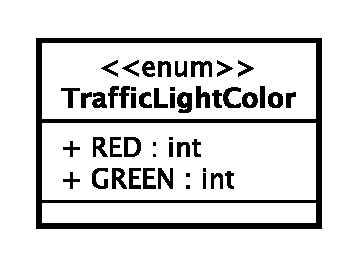
\includegraphics[scale=0.6,keepaspectratio]{images/solution/app/backend/traffic_light_color.eps}
\caption{\pReactiveComponentStretchDecoration::TrafficLightColor}
\label{fig:sd-app-traffic-light-color}
\end{figure}
\FloatBarrier
\begin{itemize}
  \item \textbf{\descr} \\
    It represents the color of a traffic light.
  \item \textbf{\values}
  \begin{itemize}
    \item[+] \texttt{RED: int} \\
    It prohibits any traffic from proceeding.
    \item[+] \texttt{GREEN: int} \\
	It allows traffic to proceed in the direction denoted.
  \end{itemize}
\end{itemize}